\chapter{Route-Aware Edge Bundling for Visualizing Origin-Destination Trails in Urban Traffic}\label{chap:c2_intro}

The visualizations for the large amounts of Origin-destination(OD) trails always cause serious clutter issues, which can be mitigated by edge bundling techniques. 
In this chapter, we first identify inconsiderate settings of conventional kernel density estimation edge bundling (KDEEB) when applied to urban traffic data, including non-optimal kernel size and road neglect. 
Then we present route aware edge bundling (RAEB) specifically designed for the OD trails bundling, which addresses these limitations by introducing a comprehensive pipeline comprising preprocessing, bundling and evaluation processes. A series of new parameters, together with adaptions of existing ones, are employed in the pipeline.


\section{Introduction}
\label{sec:intro}

Movement can be defined as change of an object's positions or geometric attributes over time~\cite{dodge_2008_towards}.
Within a specific time period, the movement of an object can be modeled with an origin (O), a destination (D), and consecutive positions (trail) in-between.
Due to fast development of location sensing technologies, massive amounts of OD trails, such as vessel movements and taxi trips, have been collected.
Studies of OD trails have revealed many movement patterns and contributed to many applications, e.g. diseases spread control~\cite{brock_2006_scaling} and transportation planning~\cite{wang2012understanding}.

Visualizing OD trails is a hot yet challenging topic.
Conventional method that connects origins to destinations with lines~\cite{tobler_1987_experiments} can easily cause visual clutter.
To tackle the problem, methods of aggregating trails into flows are usually employed.
A number of automatic techniques have emerged, such as intelligent routing layout~\cite{phan2005flow, verbeek_2011_flow} and spatial mapping~\cite{andrienko_spatial_2011-1, guo2014origin}.
These methods are preferable for revealing overall traffic patterns for answering general questions, e.g., what are popular roads in a city? where do people head to?
However, the methods mostly ignores information of individual OD trail.
In certain scenarios such as to find abnormal people movements, additional analytics are required to complement the visualization.

Wrapping up OD trails into bundles can reveal overall traffic patterns, meanwhile keep individual OD trail.
Many bundling methods including spring-based (e.g.,~\cite{holten2009force, selassie2011divided}), image-based (e.g.,~\cite{hurter2012graph, lhuillier2017ffteb}), and geometry-based (e.g.,~\cite{holten2006hierarchical, cui2008geometry}), have been proposed.
These techniques have been successfully employed for many different datasets such as Internet connections and migrations.
In these data, it is flexible to manipulate edges as long as node connections are kept.
This, however, does not hold for OD trails in urban traffic data.
In a city, humans and vehicles are moving along roads, and many activities including traffic jams and accidents, are happening on roads.
Hence, OD trails are constrained by road networks.
Trail information is equally, if not more, important as ODs for urban traffic data.

Among various edge bundling methods, kernel density estimation (KDEEB)~\cite{hurter2012graph} is in state-of-the-art with advantages in speed and generality.
However, we identify several inconsiderate settings of KDEEB when applied to OD trails in urban traffic data, including non-optimal kernel size and road neglect.
These settings wreck applicability of KDEEB for movement visualization, which requires to preserve road network topology and to support multi-scale exploration.
This work presents a new method, namely route-aware edge bundling (RAEB), specifically designed to address the limitations.
RAEB employs a comprehensive pipeline consisting of preprocessing, bundling and evaluation processes.
A series of new parameters such as route awareness and bundling stability, which leverage advanced techniques from geography and image processing fields, are introduced.
Experiments on artificial and real-world urban traffic data show that RAEB can generate more realistic results, meanwhile achieve fast computation speed comparable to KDEEB.

\vspace{1.5mm}
The primary contributions of this work include:

\begin{itemize}

\item
We develop a new edge bundling method of RAEB, which includes a comprehensive pipeline consisting of preprocessing, bundling, and evaluation processes. 

\item
We adapt existing parameters in KDEEB, and introduce a series of new parameters, to better fit OD trails in urban traffic.

\item
We conduct several experiments using artificial and real-world urban traffic data to demonstrate effectiveness of RAEB. 
\end{itemize}
% \vspace*{-1mm}
\section{Related Work}
\label{sec:related_work}

This section discusses previous studies closely related to our work.

%===============================================
\subsection{Street View Analysis}
GSV system provides high quality and accurate panoramic images of hundreds of cities~\cite{anguelov2010google}.
In recent years, researchers studying human-scale urban forms have utilized GSV images as a new and convenient data source. 
For example, researches have shown that the analysis of GSV images can be used to audit neighborhood environments~\cite{rundle_2011_using}, quantify street greenery~\cite{li_2015_accessing}, and predict street safety~\cite{Naik_2014_streetscore}.
Nonetheless, the majority of these studies face scalability issues given their focus on either a particular feature~\cite{li_2015_accessing} or a small area~\cite{rundle_2011_using, Naik_2014_streetscore, li_2015_accessing}.
Thees issues can be addressed by incorporating deep learning techniques, which can be used to summarize city landscapes~\cite{doersch2015makes} and estimate the demographic makeup of a country~\cite{gebru2017using}.

In this work, we collect $\sim$1.7 million GSV images of four representative mega-cities, and apply a deep learning technique~\cite{Badrinarayanan_2015_segnet} to automatically extract desired urban forms from the collected images.
More importantly, we develop an effective visual analytics tool for urban planners to explore human-scale urban forms.

%===============================================
\subsection{Urban Data Visualization}
Vast amounts of urban data, including traffic~\cite{ferreira_visual_2013, wang_2013_visual}, social media~\cite{xu_2013_visual, chen_2015_interactive}, environment~\cite{ferreira_2011_birdvis}, and simulated urban spaces~\cite{vanegas_2009_visualization}, have been collected in an urban context.
Big urban data brings in unprecedented opportunities for evidence-based urban design, and visualization systems can assist domain experts in finding evidence from the data.
A systematic overview of visualization systems can be found in~\cite{zheng_2016_visual}.

Qu et al.~\cite{qu_2007_visual} presented a comprehensive visualization system for the analysis of a city's air pollution that affects the daily lives of residents.
Their system integrates parallel coordinates and scatterplots to show relationships between high-dimensional air pollutants.
In addition to air pollution, landmark visibility is related to the daily experience of a city's residents.
Ortner et al.~\cite{ortner_2016_vis-a-ware} visually compared the effects of candidate buildings on landmark visibility from various viewpoints.
In this system, users can select a series of ranking schemes, and candidate buildings are then automatically sorted.
Similar to our present work, Arietta et al.~\cite{arietta_2014_city} associated visual elements with city attributes, including violent crime rates and housing prices.
They developed various prototype visualizations, such as the visual boundary of urban neighborhoods.

% \vspace{2mm}
Although different data are explored, these visualizations similarly employ CMVs, because urban data typically exhibits both spatial information and multi-dimensional attributes.
Our system also adopts this empirical approach.
In addition, to address specific domain problems, we develop effective visualization techniques, including a novel parallel coordinates enhanced with street layouts.

%===============================================
\subsection{Multivariate Geographical Data Visualization}
Visualizing multivariate data is a hot topic in the visualization field.
Numerous conventional approaches to this topic have been developed, and can be classified into two groups:
1) employing visualization techniques, such as parallel coordinates plot (PCP), scatterplot matrix, and start coordinates;
and 2) projecting data points onto a two- or three-dimensional visual space that can be directly plotted on a screen, such as multidimensional scaling and principal component analysis.
All these approaches have pros and cons.
For example, although PCP presents all dimensional attributes without information loss, it can easily generate visual clutter with big data and pairwise correlations can only be shown on two nearby coordinates~\cite{heinrich_2012_state}.
Many improvements have been developed to address these issues.
These improvements include edge bundling to reduce visual clutter~\cite{zhou2008visual, holten_2010_evaluation}, and hierarchical data clustering and the navigation of resulting structures~\cite{fua1999hierarchical, zhao_2012_structure}.
% ., and sort dimensions in order based on their correlations~\cite{zhao_2012_structure, wu_2015_telcovis}.

When multivariate data is dependent upon locations, the analytical tasks become more complex because geographical information needs to be revealed.
Turkay et al. developed \textit{Attribute Signature}~\cite{turkay_2014_attribute}, which employs a geographical map and small multiples of multivariate attributes to show geographic variability in attribute statistics.
Goodwin et al.~\cite{goodwin_2016_visualizing} further explored multivariate geographical data across scales by adopting new designs to show correlation, scale, and geographical information.
The frameworks proposed by both studies can be generalized to explore multivariate geographical data.

In this work, human-scale urban forms to be explored are also multivariate geographical data: the features are in six dimensions and they are dependent on locations.
We leverage the advantages of scatterplot matrix and PCP for different analytical tasks.
Specifically, we employ scatterplot matrix for exploring features at city- and region scales given that it can effectively reveal correlations between all pair-wise features.
We also arrange the views in a way similar to \textit{Attribute Signature}~\cite{turkay_2014_attribute}, i.e., geographical information is presented on maps and multivariate attributes in small multiples. 
In addition, we develop a novel PCP enhanced with a themeriver plot, which fits better with the analytical task of showing feature variations along street layout at street-scale.

%===============================================
\subsection{Comparative Visualization}
Gleicher et al.~\cite{gleicher_2011_visual} classified techniques for visual comparison into three categories:
1) Juxtaposition, i.e., presenting objects next to each other. 
For example, NodeTrix~\cite{yang_2017_blockwise} arranges two human brain networks side-by-side. 
2) Superposition, i.e., presenting multiple objects on top of one another.
Typical examples are time-series line graphs that plot the changes in several variables over time in the same coordinate system.
3) Explicit encoding, i.e., presenting differences or correlations between objects visually.
For instance, the bivariate density map is employed in~\cite{zeng_2017_visualizing} to show the relationship between departure and arrival movements over space.
In practice, these techniques are combined to address complex analytical tasks.

Our work adopts juxtaposition that arranges maps of two AOIs/streets side-by-side (Fig.~\ref{fig:teaser}(b) \& (d)), and superposition to compare multivariate features of two AOIs/streets in the same coordinate system (Fig.~\ref{fig:teaser}(c) \& (e)).

\if 0
\subsection{Human-scale Urban Form}
Though human-scale urban form is defined recently~\cite{long_2016_human-scale}, discussions of the concept in urban planning and designing have a long history that can be traced to 1960s.
A series of pioneering studies~\cite{jacobs_1961_life, gehl_1971_life} claimed the positive effects of human-scale urban form in designing high-quality urban space.
Among various types of human-scale urban form, the visible one is particularly important as human beings tend to pay most attentions to surroundings that can be directly seen~\cite{gehl_1971_life}. 

Accompanying with the raising of big open data, e.g., GSV images, researches in studying visible human-scale urban form are focusing on quantitatively measuring the related features nowadays. 
For example, researches have shown that analyzing GSV images can audit neighborhood environments~\cite{rundle_2011_using}, quantify street greenery~\cite{li_2015_accessing} and predict street safety~\cite{Naik_2014_streetscore}.
Nonetheless, most of these researches got scalability issues as they focused on either a particular feature or a small area.
The issues can be addressed by incorporating deep learning techniques, by which recent studies have shown its applicability in summarizing landscape of a city~\cite{doersch2015makes} and even estimating demographic makeup of a country~\cite{gebru2017using}.

\vspace{2mm}
In this work, we first identify the important features of visible human-scale urban form, then collect millions of GSV images across four representative mega-cities, and apply a deep learning technique - SegNet~\cite{Badrinarayanan_2015_segnet} - to automatically label related features in the images.
More importantly, we develop an effective visual analytical tool for urban planners to explore the analysis on demand.

\fi

\if 0
\subsection{Street view images analysis}

Google street view(GSV) is a well know system that provides panoramic images in hundreds of cities of more than 20 countries to millions of googles users. During the past 15 year, GSV system can provide a good quality and accurate images service, and more and more researchers begin to focus on this data source\cite{anguelov2010google}. GSV is considered as a novel and convenient way to collect environmental information and has been utilized in a broad range of research domains including ecology, geography, archeology, urbanology and even some social science. 

In recent years, the researchers in the ecology field found that the GSV images was an alternative way to observe the natural environment. Olea et al. \cite{olea2013assessing} discussed that the GSV images could be a good data source to assess the habit of some cliff living animals and the using of both of these two methods could be highly useful as a coarse-scale assessment method over large geographic areas. Hardion et al.\cite{hardion2016species} proposed a  time and cost-effective solution using the geo-located street view images in the analysis of species distributions. In the discipline of urbanology and sociology, GSV has been used in the virtual audit of different physical environment\cite{clarke2010using, rundle2011using, kelly2013using, vanwolleghem2014assessing} in the city. These methods has the potential to significantly reduce the costs and time of collecting data and can be well adapted in the large geo-scale research. 

Even though the GSV images could be adapted in different research areas, in the most instance, the observation of environment is still conducted by human beings. Nowadays, fast developed of deep learning techniques has been widely used in image processing, many research has considered the automatic methods to further reduce the human cost. Doersch et al.\cite{doersch2015makes} analyzed millions of image from GSV to extract the visual features commonly occurred to summary the landscape of a city. Timnit et al.\cite{gebru2017using} also proposed a method use deep learning techniques and GSV images to estimate teh demographic makeup of United States.
\fi

\section{Problem Statement and System Overview}
\label{sec:overview}

This section briefly describes KDEEB algorithm, followed by a discussion of inconsiderate settings when applied to OD trails in urban traffic.
An overview of RAEB is presented at the end.

\begin{figure}[t] 
	\centering
	\includegraphics[width=0.495\textwidth]{fig2_kernel_size/kernel_size}
	\vspace{-5mm}
	\caption{KDEEB applied to taxi trips in Manhattan with different kernel sizes $p_r$: (a) 120, (b) 80, (c) 40, and (d) 20.
	More detailed bundles are generated with smaller $p_r$.}
	\label{fig:kernel_size}
	\vspace{-5mm}
\end{figure}

%%%%%%%%%%%%%%%%%%%%%%%%%%%%%%%%%%%%%%%%%%%%%%%%%%%%%%%%%%%%%%%%%%%%
%%%%%%%%%%%%%%%%%%%%%%%%%%%%%%%%%%%%%%%%%%%%%%%%%%%%%%%%%%%%%%%%%%%%

\subsection{KDEEB Algorithm}
\label{ssec:kdeeb}
KDEEB is a fast edge bundling method for visualizing dense graphs.
It employs a general pipeline with edge sampling, splatting, gradient estimation, edge advection, and bundle smoothing.
In edge sampling step, an edge $\textbf{e}_i$ is divided into uniformly-sampled polylines, i.e., $\textbf{e}_i = \{\textbf{x}_j\}$, with user-given sampling step $\sigma$.
After that, KDEEB computes a density map $\rho : \mathbb{R}^2 \rightarrow \mathbb{R}^+ $as

\vspace{-4mm}
\begin{equation}\label{eq:kernel_density_estimation}
\rho(\textbf{x} \in \mathbb{R}^2) = \sum_{\textbf{y} \in D} K (\frac{\|\textbf{x}-\textbf{y}\|}{p_r})
\end{equation}

where $K$ is a parabolic radial kernel and $p_r$ is kernel radius.
Next, each edge sampling site $\textbf{x}_j$ is advected to a new position $\textbf{x}'_j$ as:

\vspace{-5mm}
\begin{equation}\label{eq:advecting_points}
\textbf{x}'_j = \textbf{x}_j + p_r \frac{\nabla \rho}{||\nabla \rho||}
\end{equation}

Finally, a smoothing function is applied on $\textbf{x}_j$ to remove jitters created by the advection step.
These steps are repeated $p_n$ times until stable bundles are generated.

\vspace{2mm}
\noindent
\textit{Parameter Setting}.
KDEEB requires several parameters to be preset by users.
Following settings are recommended~\cite{van2016cubu}:
\begin{itemize}

\item 
Kernel radius $p_r$: Initial value set to 5\% of graph drawing size.
A constant decay ratio $\lambda$ in [0.5, 0.9] is applied to $p_r$ at each bundling iteration $n$.

\item
Bundling iteration $p_n$: An integer in between 10 to 15.

\end{itemize}

\begin{figure*}[t]
	\centering
	\includegraphics[width=0.995\textwidth]{fig3_framework/framework2.pdf}
	\vspace{-3mm}
	\caption{Overview of RAEB pipeline.
	Our method mainly consists of three phases: \textit{Preprocessing} for creating a proper initial layout, \textit{Bundling} for bundling input OD trails, and \textit{Evaluation} for generating a stable bundle structure.}
	\label{fig:framework}
	\vspace{-4mm}
\end{figure*}

%%%%%%%%%%%%%%%%%%%%%%%%%%%%%%%%%%%%%%%%%%%%%%%%%%%%%%%%%%%%%%%%%%%%
\subsection{Problem Identification}
The parameter settings are recommended for general graphs that consist of fixed nodes and connections between them.
For such a graph, it is free to manipulate node connections into smooth polylines.
However, when applied to OD trails in urban traffic data, KDEEB encounters the following issues.

\begin{itemize}
\item
\textit{P1: Non-optimal Kernel Radius}.
Kernel radius $p_r$ in KDEEB is solely based on graph drawing size, while ignores geometric properties of road network.
Figure~\ref{fig:kernel_size} presents KDEEB results generated with different kernel sizes for taxi trips in Manhattan: 120, 80, 40, and 20 in (a) - (d), respectively.
Sizes for graph drawing are all 720$\times$1440, thus KDEEB would recommend $p_r$ = 80 as 5\% of graph graphing size.
However, smaller $p_r$ generate more detailed and visual appealing bundles, comparing Figure~\ref{fig:kernel_size}(b) to (c) \& (d).
This happens because most space in graph drawing are not utilized, due to the long and thin shape of Manhattan island.
In addition, urban traffic can unevenly spread in a city, such as Shenzhen taxi data (Section~\ref{ssec:study3}), making small $p_r$ preferable.

\vspace{1mm}
\item
\textit{P2: Road Neglect}.
Urban traffic are moving along roads in a city, thus OD trails should be constrained to roads in a city.
However, KDEEB represents each OD connection with a direct line, while ignores information about the road network.
Thus, resulting bundles can be displaced far away from the roads.
This can cause impression of traffic moving in wrong positions, such as those bundles in between Manhattan and Brooklyn (Section~\ref{ssec:study1}).
The displacements can also add difficulty to mentally map original OD trails with resulting bundle lines.
\end{itemize}

\vspace{2mm}
\noindent
Besides, KDEEB lacks a quantitative method to automatically terminate bundling iterations.

\begin{itemize}
\item
\textit{P3: Preset Bundling Iterations}.
KDEEB is an image-based edge bundling method. 
Most of these bundling methods generate bundling results in an iterative way. 
The number of bundling iterations $p_n$ is preset based on practical experience: 10 in KDEEB~\cite{hurter2012graph}, while 15 in CUBu~\cite{van2016cubu}.
The numbers are chosen because tight and stable bundles are generated.
However, these conditions are rather subjective, which can vary among individuals and may be affected by other parameters like image size and sampling step.
\end{itemize}

%%%%%%%%%%%%%%%%%%%%%%%%%%%%%%%%%%%%%%%%%%%%%%%%%%%%%%%%%%%%%%%%%%%%
\subsection{RAEB Overview}
We develop route-aware edge bundling (RAEB), a comprehensive edge bundling method specifically designed for visualizing OD trails in urban traffic.
As illustrated in Figure~\ref{fig:framework}, RAEB pipeline mainly consists of three parts: \textit{Preprocessing}, \textit{Bundling}, and \textit{Evaluation}.

In \textit{Preprocessing}, RAEB first generates a simplified road network from the input one such as open street map (OSM).
Raw OD trails are mapped onto simplified road network using map matching algorithms.
Together with urban traffic information, simplified road network can be organized in a hierarchical route structure.
OD trails can be abstracted accordingly depending on a new parameter of route awareness defined by users.
A value for kernel size is also measured based on geometric property of the route structure.

The abstract OD trails are passed into \textit{Bundling} stage as input graph.
Bundling process is an image-based approach similar to KDEEB workflow.
Specifically, we discard the preset parameter of bundling iteration $p_n$ in KDEEB.
Instead, we introduce a new parameter of bundling stability, which is measured as normalized mutual information between images generated by two consecutive iterations.
The measurement is done in the \textit{Evaluation} stage.
If bundling stability reaches a threshold, we terminate the bundling iteration and export a final image.
Besides, we measure Fréchet distance between generated bundles to OD trails mapped on the road network.
The measurement complements final image with a quantitative metric that reveals quality of a bundling method.

\section{Preprocessing}
\label{sec:preprocess}
%%%%%%%%%%%%%%%%%%%%%%%%%%%%%%%%%%%%%%%%%%%%%%%%%%%%%%%%%%%%%%%%%%%%%%%%%%%%%%%%%%%%%%%%%%%%%%%%%%

This work leverages both OD trails and road network to improve edge bundling quality.
This section introduces major steps in \textit{Preprocessing} stage, including: map matching, hierarchical road structure construction, and trail abstraction.

%%%%%%%%%%%%%%%%%%%%%%%%%%%%%%%%%%%%%%%%%%%%%%%%%%%%%%%%%%%%%%%%%%%%
\subsection{Basic Traffic Concepts}
\textit{Road Network}:
A road network can be modeled as a directed graph $\bar{G} = (\bar{V}, \bar{E})$, where $\bar{V}$ is the set of nodes in $\bar{G}$ and $\bar{E}$ is the set of edges connecting nodes in $\bar{V}$.
Degree of a vertex $\bar{v}$, denoted as $deg(\bar{v})$, indicating the number of edges connected to $\bar{v}$.
By this, a vertex $\bar{v} \in \bar{V}$ can be classified as an endpoint with $deg(\bar{v})=1$, a midpoint with $deg(\bar{v})=2$, or an intersection with $deg(\bar{v})>2$.
To facilitate computation, we can simply $\bar{G}$ into a simplified graph $G = (V, R)$, where $V$ is the union of endpoints and intersections, and $R$ is a set of links connecting nodes in $V$.
Each link $r$ represents a sequence of $n$ consecutive nodes in $\bar{V}$:

\vspace{-7mm}
\begin{equation}
  \begin{aligned}
  	r &:= \bar{v}_1 \rightarrow \bar{v}_2 \rightarrow ... \rightarrow \bar{v}_n, \,\,\, \forall \bar{v}_i \in \bar{V}
  \end{aligned}
\end{equation}

\vspace{-2mm}
\noindent
where $\bar{v}_1$ and $\bar{v}_n$ are endpoints or intersections, while the other nodes are midpoints.
For the sake of clarity, we use the term \textit{route} to describe such a link.
Computation tasks, including shortest path query and map matching, are performed on the simplified graph $G$.

\vspace{1mm}
\noindent
\textit{Urban Traffic}:
Thanks to open data campaign, many urban traffic data are available nowadays.
Typically, raw urban traffic data can come in either of the following forms:

\begin{itemize}
\item
\textit{UT-1}: origin and destination locations only, such as New York taxi trips~\cite{ferreira2013visual} and Singapore public transportation rides~\cite{zeng_2015_visualizing}.
Such a raw trip $t_{raw}$ can be represented as $t_{raw} := l_o \rightarrow l_d$, where $l_o$ and $l_d$ represent origin and destination locations, respectively.

\item
\textit{UT-2}: a sequence of GPS positions, such as Stuttgart scooter fleet~\cite{kruger_trajectorylenses_2013} and Hangzhou taxi trips~\cite{wang_2014_visual-reasoning}.
Such a raw trip $t_{raw}$ can be represented as $t_{raw} := l_1 \rightarrow l_2 \rightarrow ... \rightarrow l_n$, where $l_i \subset \mathbb{R}^2$. $l_1$ and $l_n$ are origin and destination, i.e., $l_o$ and $l_d$.
\end{itemize}

Both forms of urban traffic data can be generalized as a traffic graph $G_t = (L, T)$, where $L$ is the set of locations and $T$ is the set of trips represented as sequential connections of locations.

%%%%%%%%%%%%%%%%%%%%%%%%%%%%%%%%%%%%%%%%%%%%%%%%%%%%%%%%%%%%%%%%%%%%%%%
\subsection{Map Matching}
\label{section:edge_matching}

Constraining movements over an underlying road network, i.e., mapping traffic graph $G_t := (L, T)$ to road network $G := (V, R)$, is usually a preliminary step for urban traffic analysis.
This is necessary.
First, recorded locations get errors due to imprecise GPS localization, while road network is precise and constant.
Second, $G_t$ can be much more complex than $G$:
Taking New York traffic for an example, there are over millions of taxi trips per day, resulting in millions of locations $L$, yet its simplified road network contains less than 100K routes.
Therefore, map matching can enrich effective analysis and visualization.

There are many map matching methods available, including shortest path, minimum turns, and ST-matching~\cite{lou_2009_map} for GPS traces.
These methods are preferable for different dataset.
We employ the following methods for corresponding urban traffic.

\begin{itemize}

\item
For \textit{UT-1}, i.e., $t_{raw} = l_o \rightarrow l_d$, we first find corresponding closest nodes $v_o \in V$, $v_d \in V$ for $l_o$ and $l_d$ respectively.
After that, we search for the shortest path between $v_o$ and $v_d$ in $G$.

\item
For \textit{UT-2}, i.e., $t_{raw} = l_1 \rightarrow l_2 \rightarrow ... \rightarrow l_n$, we use ST-matching algorithm, which considers not only spatial features of road network, but also temporal constraints.
The method was later visually investigated and optimized with an interactive interface~\cite{kruger_2018_visual}.
\end{itemize}

Both methods return a sequence of routes $r_1 \rightarrow r_2 \rightarrow ... \rightarrow r_n$ in $G$ for each OD trail $t_{raw}$.
We then combine the routes with origin ($l_o$) and destination ($l_d$) locations of $t_{raw}$.
Thus, both types of $t_{raw}$ are converted to the same map matching form. 

\vspace{-7mm}
\begin{equation}
  	\begin{aligned}
t_{map} := l_o \rightarrow r_1 \rightarrow r_2 \rightarrow ... \rightarrow r_n \rightarrow l_d.
 	\end{aligned}
\end{equation}
\vspace{-1mm}

Here the OD trail's origin $l_o$ and destination $l_d$ are kept.

%%%%%%%%%%%%%%%%%%%%%%%%%%%%%%%%%%%%%%%%%%%%%%%%%%%%%%%%%%%%%%%%%%%%%%%%%%%%%%%%%%%%%%%%%%%%%%%%%%
\subsection{Hierarchical Route Structure Construction}
\label{ssec:hiera_road}

\begin{table}
	\centering
	\begin{tabular}{|c|c|c|}
	\hline
	Category & Exemplary OSM Indicator & Score ($r_{hier}$)  \\ \hline
	Expressway & motorway, trunk & 1 \\ \hline
	Trunk Road & primary, motorway\_link& 0.75 \\ \hline
	Secondary Road & secondary, tertiary & 0.5 \\ \hline
	Branch Road & unclassified, residential & 0.25 \\ \hline
	\end{tabular}
	\vspace{1mm}
	\caption{Route hierarchy, OSM indicator and hierarchy score} \label{tab:sometab}
	\label{table: road_score}
\vspace{-6mm}
\end{table}

A road network is usually designed in hierarchical levels to avoid dense direct connections among regions.
This inspires us to construct a hierarchical route structure to benefit edge bundling.
Although urban roads are organized hierarchically, it does not consider OD trails.
This work makes use of the following attributes of a route $r$ in $G := (V, R)$ to construct a hierarchical route structure.

\vspace{1mm}
\noindent
\textit{Route length} ($len(r)$).
Visual appearance of each OD trail is determined by its routes on road network.
Longer a route, more it will affect the visual appearance.
Thus an important component affecting route hierarchy is route length.
Here, $len(r)$ is measured in Euclidean space and normalized over the whole road network.

\vspace{1mm}
\noindent
\textit{Road hierarchy} ($hier(r)$).
Urban roads are classified into hierarchies: freeways, arterials, collectors, and local roads.
Similar descriptions can also be found elsewhere~\cite{wang_2014_visual-reasoning}.
A higher level usually indicates faster traffic speed and less access to property.
OSM provides more detailed indicators of road hierarchy, e.g., trunk, primary, tertiary, etc.
To keep consistent, we classify these indicators into four hierarchies.
A route $r$ in each hierarchy is assigned an score according to Table~\ref{table: road_score}. 

\vspace{1mm}
\noindent
\textit{Flow magnitude} ($flow(r)$).
Flow magnitude measures how many OD trails pass through a route $r$.
The previous two factors purely rely on road network, while $flow(r)$ reflects the importance of a route in consideration of OD trails.
Here, $flow(r)$ is measured by counting how many mapped OD trails passing through $r$, and then normalized. 

\vspace{2mm}
By this, each route can be represented by a vector $V(r) := <len(r), hier(r), flow(r)>$.
Score of a route $score(r)$ can be measured as $score(r) = \sum w_i \times V(r)_i$, where the weights $w_i (i = 1, 2, 3)$ controls how much each attribute affects route weight.
We choose 0.3, 0.1, and 0.6 in this work, which highlights the importance of flow magnitude.
In the end, all routes are sorted in descending order according to their weights.
The routes $R$ are further subdivided into multiple hierarchical levels $R^1$, $R^2$, ..., $R^n$.
Each level of routes accounts for top-k routes.

\begin{figure}[t]
	\centering
	\includegraphics[width=0.7\textwidth]{figure/edgebundling/fig4_od_abstraction/OD_Abstraction.pdf}
	\vspace{-3mm}
	\caption{Illustration of hierarchical route structure and OD trail abstraction:
	(a) Three route levels are constructed colored in blue, purple and green, repsectively; a raw OD trail is abstracted in accordance to route (b) level-3, (c) level-2, and (d) level-1.}
	\label{fig:road_hierarchy}
	\vspace{-1mm}
\end{figure}

%%%%%%%%%%%%%%%%%%%%%%%%%%%%%%%%%%%%%%%%%%%%%%%%%%%%%%%%%%%%%%%%%%%%%%%%%%%%%%%%%%%%%%%%%%%%%%%%%%
\subsection{Trail Abstraction}
\label{section: trail_abstraction}

\textbf{P2} states that road network is omitted in original KDEEB, which can lead to wrong depiction in geographical space and poor support of multi-scale exploration.
We introduce a new parameter of route awareness $p_{ra}$, which defines the level of trail abstraction, to tackle this issue.
Higher $p_{ra}$ indicates that more details of OD trails should be preserved.
Given a hierarchical route structure in $n$ levels, $p_{ra}$ can range from 0 to $n$.
If $p_{ra}$ is set to zero, OD trails will be abstracted to straight lines connecting ODs directly.
If $p_{ra}$ is set to $n$, no abstraction will be applied.
If $p_{ra}$ is set to a value $m$ in [1, $n-1$], routes in level-1 to level-$m$ will be preserved.

Figure~\ref{fig:road_hierarchy}(a) presents an exemplary road network with a hierarchical route structure.
The routes are categorized into three levels: blue thick lines for level 1, purple medium lines for level 2, and green thin lines for level 3.
Figure~\ref{fig:road_hierarchy}(b-d) illustrates an example of how a raw OD trail of $l_o \rightarrow r_1 
\rightarrow...\rightarrow r_6 \rightarrow l_d$ can be abstracted in accordance to the hierarchical route structure shown in Figure~\ref{fig:road_hierarchy}(a).
In Figure~\ref{fig:road_hierarchy}(b), $p_{ra}$ is set 3, and all routes are preserved.
In Figure~\ref{fig:road_hierarchy}(c), $p_{ra}$ is set 2, so route $r_1$ and $r_2$ will be merged together as they are both level-3 routes.
In Figure~\ref{fig:road_hierarchy}(d), $p_{ra}$ is set 1, thus only route $r_4$ will be kept.
\section{Bundling Method}
\label{sec:bundling}
\begin{algorithm}[h]
	\caption{KernelSizeMeasurement}\label{al:kernel_size_measurement}
	\begin{algorithmic}[1]
		\Require Top \textit{N} sorted routes as polyline list $\textbf{P} = \{P_1, ..., P_N\}$
		\Ensure Initial kernel size $p_r$		
		\State Let $d$[ ][ ] denote distance between polyline pairs
		\For {i = 1 to $N$}
		\For {j = i + 1 to $N$}
		\State $d$[i][j] = $d$[j][i] = DiscreteFrechetDistance($P_i$, $P_j$)
		\EndFor
		\EndFor
		\State Let \textbf{C} denote a list of polyline clusters;
		\State \textbf{C} = $DBSCAN(\textbf{P}, eps, minNum)$;
		\State $C_{max}$ = $argmax_{|C_i|}(C_i | C_i \in \textbf{C})$;
		\State Initialize $d_{geo} = 0$;
		\State Let $count = |C_{max}| \times (|C_{max}| - 1)$;
		\ForEach {$P_i \in C_{max}$}
		\ForEach {$P_j \in C_{max}$ \&\& $P_i \neq P_j$}
		\State $d_{geo}$ = $d_{geo}$ + $d$[i][j] / count;
		\EndFor
		\EndFor
		\State $p_r$ = ToDrawingSpace($d_{geo}$ / 2); \\
		\Return $p_r$
	\end{algorithmic}
\end{algorithm}


RAEB adapts KDEEB bundling algorithm~\cite{hurter2012graph} to better reveal topology of urban traffic.
This sections presents amendments employed by RAEB, including kernel size measurement and density map generation.



%%%%%%%%%%%%%%%%%%%%%%%%%%%%%%%%%%%%%%%%%%%%%%%%%%%%%%%%%%%%%%%%%%%%%%%%%%%%%%%%%%%%%%%%%%%%%%%%%%
%%%%%%%%%%%%%%%%%%%%%%%%%%%%%%%%%%%%%%%%%%%%%%%%%%%%%%%%%%%%%%%%%%%%%%%%%%%%%%%%%%%%%%%%%%%%%%%%%%
\subsection{Optimal Kernel Size}
\label{ssec:kernel_size}
KDEEB only considers the size of graph drawing when determining kernel size.
This strategy may not be optimal for bundling OD trails in urban traffic (\textit{P1}).
Ideally, the chosen kernel size should be able to bundle closely-related OD trails (e.g., movements on bi-directional roads), while separate loosely-correlated OD trails (e.g., movements on two different highways).

To address \textit{P1}, both graph drawing size and geometric property of road network should be considered.
We develop an automatic process for measuring initial kernel size, as outlined in Algorithm~\ref{al:kernel_size_measurement}.
Here, top $N$ routes are extracted from \textit{Preprocessing} stage.
The routes are treated as a polyline list \textbf{P}, and inputted into the algorithm.
Pair-wise distance between each pair of ploylines are computed. 
Then a DBSCAN algorithm is applied to group the polylines into polyline clusters \textbf{C}.
The cluster with maximum number of polylines is extracted, and denoted as $C_{max}$.
Average geographical distance $d_{geo}$ is computed for polylines in $C_{max}$.
Finally, half of $dist_{geo}$ is converted to $p_r$ in graph drawing space, and $p_r$ is returned as the initial kernel size.

Basically, the algorithm first computes average geographical route distance in the top $N$ routes, and then converts the distance to graph drawing space.
$N$ should not be too small that the routes are not representative for the whole road network; meanwhile, it should not be too big to overlap route awareness.
From our experiments, we find 1\% of whole route size is appropriate for $N$.
Besides, another important factor is the distance metric between two polylines.
Here, we choose discrete Frechet distance, which measures similarity of two polylines considering both locations and ordering of the points along the polylines.
The metric is one of the most popular methods for movement analysis~\cite{gudmundsson2011computational}, and can be computed efficiently~\cite{eiter_1994_computing}.

%%%%%%%%%%%%%%%%%%%%%%%%%%%%%%%%%%%%%%%%%%%%%%%%%%%%%%%%%%%%%%%%%%%%%%%%%%%%%%%%%%%%%%%%%%%%%%%%%%
%%%%%%%%%%%%%%%%%%%%%%%%%%%%%%%%%%%%%%%%%%%%%%%%%%%%%%%%%%%%%%%%%%%%%%%%%%%%%%%%%%%%%%%%%%%%%%%%%%
\subsection{Density Map Generation}
KDEEB omits trail information (\textit{P3}), as it connects ODs with directed lines.
We aim to keep bundles close to OD trails on road network.
More specifically, in \textit{Preprocessing} stage, each OD trail is abstracted into a sequence of artificial directed lines and real routes in road network.
The artificial directed lines are free to manipulated, while we would like to keep the bundle layout spatially close to the real routes.
In addition, it is preferable to keep the bundling paradigm of advecting sampling sites towards high density directions.

To achieve this goal, we modify the density map generation used by KDEEB.
Let denote a list of routes $R_{aware} \subset \mathbb{R}^2$ are kept for route awareness.
Since sampling sites are advected towards their gradient directions, gradients of points along $R_{aware}$ should be either (1) zero, or (2) pointing to route direction.
To minimize effects on densities surrounding $R_{aware}$, we choose the second option.
Instead of Eqn.~\ref{eq:kernel_density_estimation}, we now use

\vspace{-7mm}
\begin{equation}\label{eq:new_density}
\rho_{od} = \rho + D(\textbf{x} | \textbf{x} \in R_{aware})
\end{equation}
\vspace{-1mm}

\noindent
where $D(\textbf{x}) \in \mathbb{R}^+$ is a constant assigned to a point $\textbf{x} \in R_{aware}$.
High $D$ value will make it more likely that gradient at $\textbf{x}$ points to the same direction with the route.

\section{Evaluation}
\label{sec:eva}

Besides introduction of \textit{Preprocessing} and adaptions in \textit{Bundling}, post hoc bundling evaluation methods are also developed in RAEB.
This section introduces these methods, including mutual information and bundle deviation measurements.

%%%%%%%%%%%%%%%%%%%%%%%%%%%%%%%%%%%%%%%%%%%%%%%%%%%%%%%%%%%%%%%%%%%%%%%%%%%%%%%%%%%%%%%%%%%%%%%%%%
\subsection{Normalized Mutual Information}
After each bundling iteration, a bundling method needs to decide whether the bundling iteration should continue or not.
KDEEB presets a bundling iteration parameter $p_n$, similar to many other bundling methods including SBEB, FTTEB, and CUBu.
$p_n$ = 10 is chosen such that the bundles converge to a stable structure.
Structure stability is basically the perception of visual similarity between images generated in two consecutive bundling iterations.
However, the perception can be easily biased by many factors, including people's color perception difference, lighting conditions, etc.
It lacks a quantitative method for measuring structure stability.

\begin{figure}[t]
	\centering
	\includegraphics[width=0.7\textwidth]{figure/edgebundling/fig5_NMI/bundle_termination.pdf}
	\vspace{-5mm}
	\caption{(left) Bundling stability $p_{bs}$ measured at each bundling iteration for different decay ratios $\lambda$, (right) visually indistinguishable images are generated at iteration 10 and 11 for $\lambda=0.9$.}
	\label{fig:nmi}
	\vspace{-1mm}
\end{figure}

%%%%%%%%%%%%%%%%%%%%%%%%%%%%%%%%%%%%%%%%%%%%%%%%%%%%%%%%%%%%%%%%%%%%%%%%%%%%%%%%%%%%%%%%%%%%%%%%%%

%%%%%%%%%%%%%%%%%%%%%%%%%%%%%%%%%%%%%%%%%%%%%%%%%%%%%%%%%%%%%%%%%%%%%%%%%%%%%%%%%%%%%%%%%%%%%%%%%%

We employ mutual information (MI) - a basic concept from information theory, as a quantitative indicator for measuring bundling stability.
Maes et al.~\cite{maes1997multimodality} introduced MI to measure statistic dependence between intensities of corresponding voxels in two medical images.
This work measures MI between images generated in consecutive bundling iterations, which are geometrically aligned.
Hence, the measurement is simplified without geometry matching. 
Let denote two input images $X$ and $Y$.
MI is computed as:

\vspace{-6mm} 
\begin{equation} \label{eq:mi}
I(X, Y) = \sum_{x}\sum_{y}p(x,y)log(\frac{p(x,y)}{p(x)p(y)}))
\end{equation}

\noindent
where $p(x)$ and $p(y)$ indicate the intensity at $x \in X$ and $y \in Y$, and $p(x, y)$ measures the joint value between $p(x)$ and $p(y)$.
MI is affected by image size, while we prefer a constant measurement for different graph drawings.
Hence, we adopt normalized MI (NMI):

\vspace{-6mm} 
\begin{equation}\label{eq:nmi}
NMI(X, Y) = \frac{2I(X,Y)}{H(X) + H(Y)} 
\end{equation}

\noindent
where $H(X) = -\sum p(x)log(p(x)))$ that measures entropy for $X$.

We introduce a new parameter of bundling stability $p_{bs}$.
$p_{bs}$ is computed in every iteration as NMI($I_n$, $I_{n-1}$), where $I_n$ and $I_{n-1}$ denote images generated at iteration $n$ and $n-1$, respectively.
Figure~\ref{fig:nmi}(left) presents NMIs at each bundling iteration for three different kernel size decay ratios $\lambda$.
It is observed that NMI increases when bundling iteration increases, and smaller $\lambda$ leads to faster NMI increment.
All NMIs pass over 0.75 around iteration 10, and reach close to 0.8 at iteration 15.
Figure~\ref{fig:nmi}(right) shows two images at iteration 10 and 11 for $\lambda$ = 0.9.
The images are hardly distinguishable from each other.
Thus, we can claim the bundling produces stable results, and the process can terminate.
In this way, we determine a threshold for $p_{bs}$ to control bundle termination.
If a bigger threshold is chosen, more stable results will be generated.

%%%%%%%%%%%%%%%%%%%%%%%%%%%%%%%%%%%%%%%%%%%%%%%%%%%%%%%%%%%%%%%%%%%%%%%%%%%%%%%%%%%%%%%%%%%%%%%%%%
\subsection{Bundle Deviation}
$p_{bs}$ is introduced for measuring visual stability of bundle layouts generated by one bundling method.
However, $p_{bs}$ is not suitable for comparing bundling quality of multiple bundling methods.
Many evaluation metrics can be used for comparing graph layouts, such as edge crossing, ambiguity, and edge direction.
These metrics are suitable for general graphs without a ground truth.
However, OD trails studied in this work are constrained in roads in a city.
We would like to keep the generated bundles close to their OD trails on the road network.
Though map matching algorithm can intrdouces errors, this work treats mapped OD trails as ground truth, instead of raw OD trails.
This is because of: for \textit{UT-1} urban traffic, only origin and destination information are recorded; for \textit{UT-2} urban traffic, accuracy of GPS positions are not perfect.

We introduce a new parameter of bundle deviation, denoted as $p_{d}$, to measure distance between final bundles and OD trails mapped on the road network.
Both bundles and OD trails can be modeled as polylines made up of sequential positions in geographical space.
Thus, the distance between them can be measured using discrete Frechet Distance.
We calculate mean distances for all bundles, and map the mean in graph drawing space.
\begin{figure}[t]
	\centering
	\includegraphics[width=0.49\textwidth]{figure/edgebundling/fig7_hierar/artifical}
	\vspace{-6mm}
	\caption{
		Left: raw 100K artificial OD trails on a hierarchical road network.
		Right: RAEB bundling result with $p_{ra}$ set to 2.
		}
	\label{fig:hier}
	\vspace{-5mm}
\end{figure}

\section{Applications}
This section presents applications of RAEB on artificial OD trails, and real-world taxi data in New York and Shenzhen.
We show advancements of RAEB over KDEEB.

\begin{figure*}[t]
	\centering
	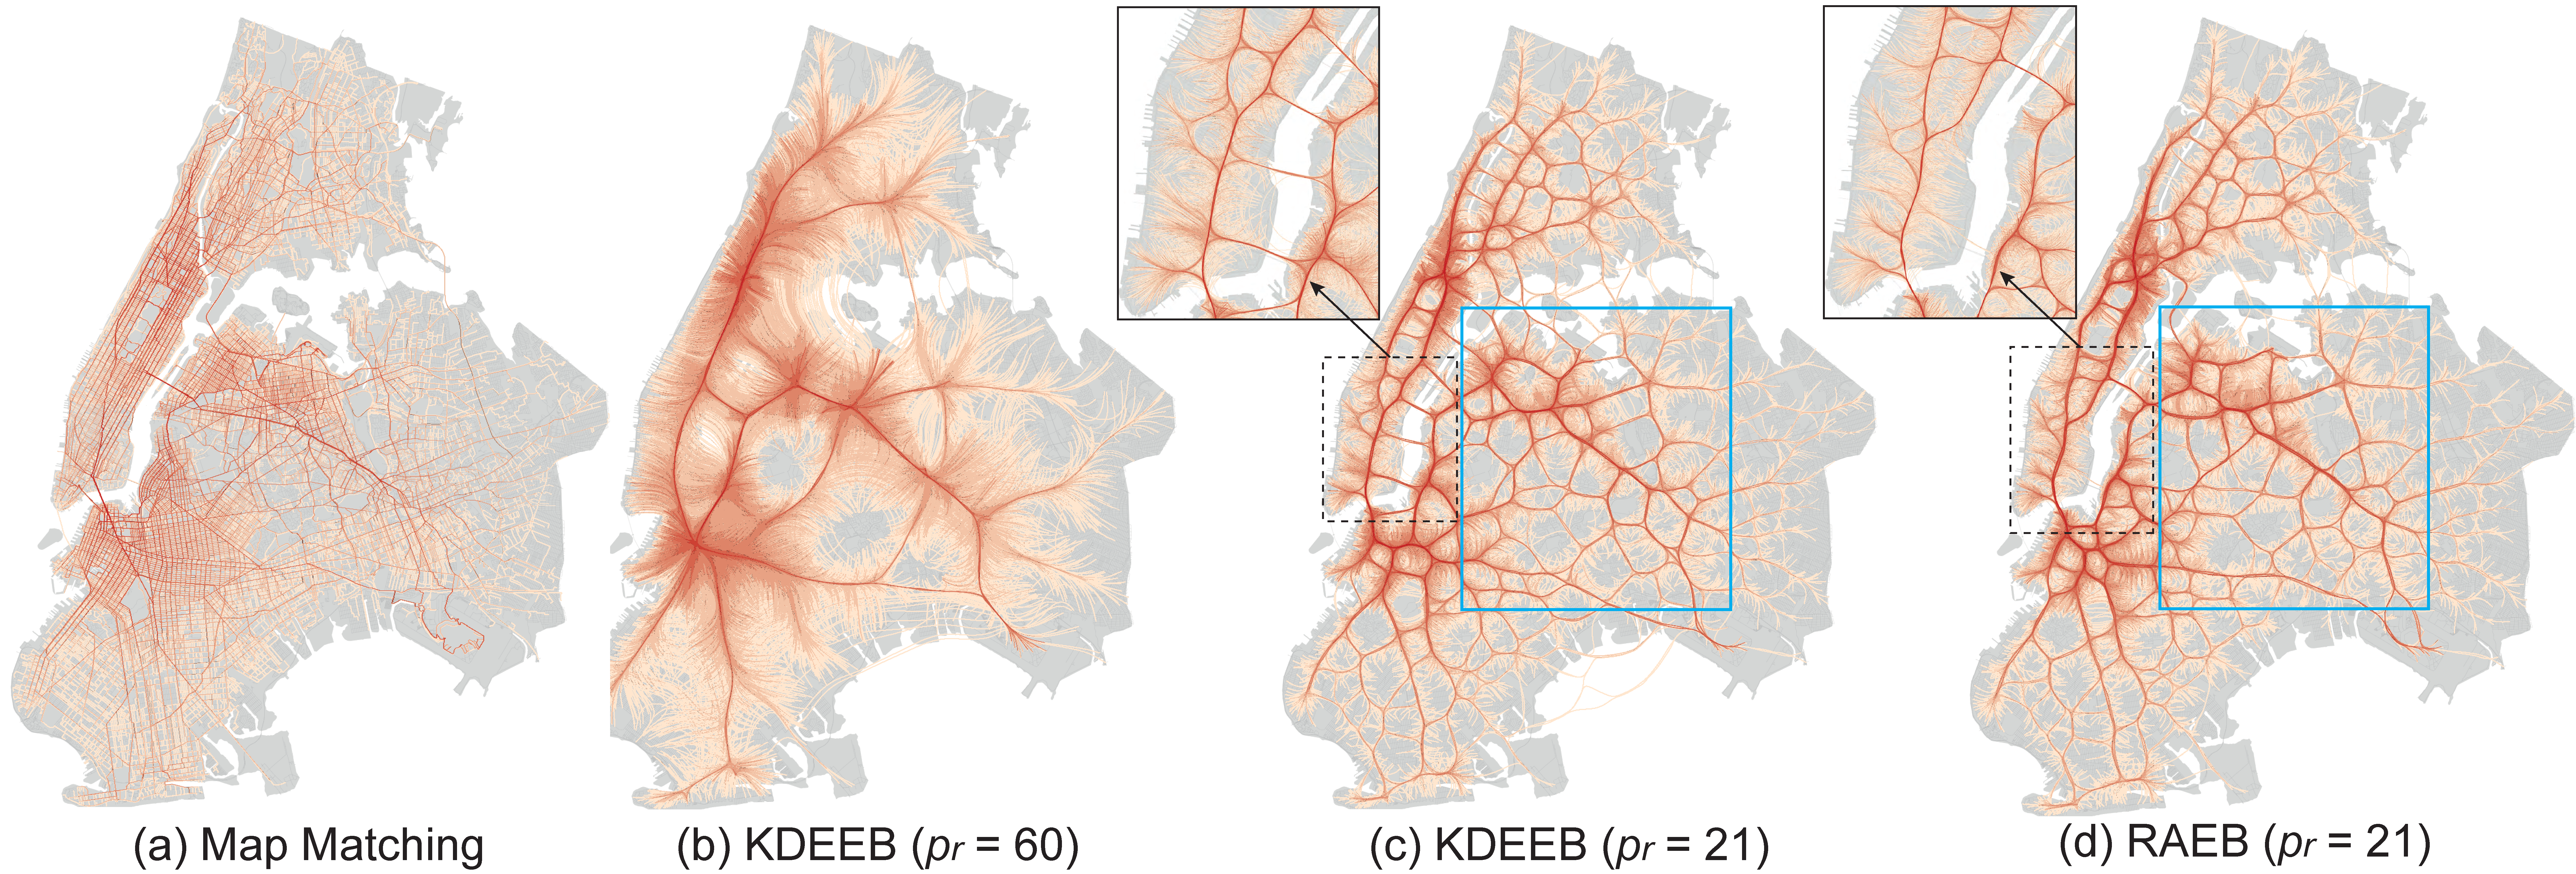
\includegraphics[width=0.995\textwidth]{figure/edgebundling/fig8_study2/NYC}
	\vspace{-2mm}
	\caption{Density maps of NYC taxi trips:
	(a) shortest paths mapped onto the road network, 
	(b) KDEEB bundles with kernel size $p_r$ = 60,
	(c) KDEEB bundles with $p_r$ = 21,
	and (d) our RAEB bundles with $p_r$ = 21.}
	\label{fig:nyc_visual}
	\vspace{-4mm}
\end{figure*}

\begin{figure}[t]
	\centering
	\includegraphics[width=0.45\textwidth]{figure/edgebundling/fig9_study2-2/NYC-zoom}
	\vspace{-3mm}
	\caption{Fine scale density maps of NYC taxi trips in Queens zone generated by (a) KDEEB, and (b) RAEB.}
	\label{fig:nyc-zoom}
	\vspace{-4mm}
\end{figure}

%%%%%%%%%%%%%%%%%%%%%%%%%%%%%%%%%%%%%%%%%%%%%%%%%%%%%%%%%%%%%%%%%%%%%%%%%%%%%%%%%%%%
\subsection{Artificial OD Trails}
\label{ssec:study1}

Our first example uses a random graph with 100K OD trails, and $5 \times 5$ grid and hierarchical reference graphs to simulate conventional road networks.
Raw OD trials and corresponding road networks are shown in the leftmost figures of Figure~\ref{fig:grid} and Figure~\ref{fig:hier}.
The OD trails are first mapped to underlying road networks using shortest path algorithm, and then both road networks are divided into three hierarchies that are colored in red, blue and green, receptively.
In the last, we apply RAEB on the OD trails, with all graph drawing sizes set to 1280$\times$1280 and initial kernel sizes $p_r$ set to 60.

In advance of KDEEB, RAEB allows to preserve route awareness by controlling parameter $p_{ra}$.
To evaluate the effects of $p_{ra}$, we set $p_{ra}$ to 0 - 3, and apply RAEB to OD trails on the grid road network as shown in the leftmost figure of Figure~\ref{fig:grid}.
The results are shown in Figure~\ref{fig:grid} (a) - (d).
In (a), $p_{ra}$ is set to 0, i.e., no route awareness will be preserved.
In this case, RAEB should be equivalent to KDEEB with other parameters the same.
The proof is demonstrated in (a), which shows smooth bundles similar to those in the original KDEEB~\cite{hurter2012graph}.
To preserve level 1 routes, we set $p_{ra}$ to 1, and the result is shown in (b).
As expected, OD trails around the red lines are bundled together with bundles following red lines, while other OD trails are bundled with bundles spreading arbitrarily in the graph drawing.
More route awareness can be preserved as we increase $p_{ra}$ to 2 and 3, as shown in Figure~\ref{fig:grid} (c) \& (d).

More importantly, route awareness $p_{ra}$ can be used to preserve topology of underlying road network.
Figure~\ref{fig:hier} (right) shows bundling result of RAEB applied to OD trails on a hierarchical road network that is shown in Figure~\ref{fig:hier}(left).
Here, $p_{ra}$ is set to 2, such that to preserve both the red and blue lines.
It is clear that the resulting bundles follow the lines, making it easy to trace OD trails.
In contrast, KDEEB will generate the same result with that in Figure~\ref{fig:grid}(a), as the underlying road network information is not used.

\begin{figure*}[t]
	\centering
	\includegraphics[width=0.995\textwidth]{figure/edgebundling/fig10_study3/shenzhen}
	\vspace{-2mm}
	\caption{
	Density maps of Shenzhen taxi trips: (a) raw GPS records are mapped onto road network, (b) KDEEB bundles trips on close aterial roads together, while (c) RAEB preserves these roads. All lines are colored according to the OD directions.
	}
	\label{fig:shenzhen}
	\vspace{-4mm}
\end{figure*}

%%%%%%%%%%%%%%%%%%%%%%%%%%%%%%%%%%%%%%%%%%%%%%%%%%%%%%%%%%%%%%%%%%%%%%%%%%%%%%%%%%%%
\subsection{New York Taxi Trips}
\label{ssec:study2}

In reality, a road network is usually much more complex, and OD trails are more dynamic than the artificial ones.
In this experiment, we further compare RAEB with KDEEB using results generated from New York taxi trips.

The road network employed in this study is extracted from OpenStreetMap (OSM) within the boundary of Manhattan, Brooklyn, Queens, and Bronx zones, where most origins and destinations are located.
The raw network consists of 133,154 nodes, 166,122 edges, and it is simplified to 97,336 routes.
The OD trails studied in this experiment are 100K taxi trips extracted from one-month trip records.
The original records consist of various attributes for each trip, including vendor id, pickup \& dropoff times and positions, and fare amount, etc.
We use the pickup \& dropoff positions, and map it onto the road network using shortest path algorithm.
Figure~\ref{fig:nyc_visual}(a) presents a density map of the mapped taxi trips.

Figure~\ref{fig:nyc_visual}(b - d) show bundling results generated by KDEEB and RAEB, with graph drawing sizes set to 1080 $\times$ 1440.
The experiment is started with KDEEB recommended settings of kernel size $p_r$ = 60 (about 5\% of graph drawing size) and $p_n$ = 10.
Figure~\ref{fig:nyc_visual}(b) shows the bundling result, which clearly presents several main bundles.
The bundles reveal primary traffic movements over the whole city.
Yet in other ways, the results are heavily bundled, missing details of road network topology.
To show more details, we measure initial kernel size considering both graph drawing and geometric property of road network as described in Section~\ref{ssec:kernel_size}.
$p_r$ is reduced to 21.
Figure~\ref{fig:nyc_visual}(c) shows the corresponding KDEEB bundling results.
More bundles are formed, in line with arterial roads in New York.
However, there are many bundles lying by non-existing roads, as those shown in the highlighted region in-between Manhattan and Brooklyn.
This illustration can cause wrong impression of bridges connecting the zones.
Figure~\ref{fig:nyc_visual}(d) shows results generated by RAEB, with $p_r$ = 21 and route awareness $p_{ra}$ = 1.
The undesirable bundles are removed by our method.

Visualization of urban traffic should support multi-scale exploration $-$ an important characteristic for movement data visualization.
In the context of this work, a good edge bundling algorithm should provide smooth transitions of bundling results at different scales.
We further evaluate multi-scale exploration by zooming into the blue region in Queens zone as in Figure~\ref{fig:nyc_visual}(c) \& (d), and applying KDEEB and RAEB on the OD trails.
The fine scale bundling results are presented in Figure~\ref{fig:nyc-zoom}(a) \& (b), respectively.
More bundles are generated by both methods, as the same effect when zooming into maps.
However, it is difficult to visually match bundles in Figure~\ref{fig:nyc_visual}(c) with those in Figure~\ref{fig:nyc-zoom}(a).
In comparison, bundles in Figure~\ref{fig:nyc_visual}(d) can be more easily identified in Figure~\ref{fig:nyc-zoom}(d).

%%%%%%%%%%%%%%%%%%%%%%%%%%%%%%%%%%%%%%%%%%%%%%%%%%%%%%%%%%%%%%%%%%%%%%%%%%%%%%%%%%%%
\subsection{Shenzhen Taxi Trips}
\label{ssec:study3}

We further evaluate the performance of RAEB using taxi trips in Shenzhen, with road network extracted from OSM.
In total, there are 161K nodes and 177K edges, and the edges are simplified to 51K routes.
The OD trails are one-week taxi trip records.
Unlike New York taxi records with only origin and destination positions, Shenzhen's data contain a sequence of GPS positions recorded in every 20 seconds.
We clean and extract in total 50K taxi trips from the records.
The trips are further mapped onto the road network using ST-matching algorithm~\cite{lou_2009_map}.

Figure~\ref{fig:shenzhen}(a) presents a graph of the map matching results in the size of 2160$\times$1280.
The lines of a trip are colored according to direction from the trip's origin to destination.
The graph shows that most taxi trips are recorded in the southern region of Shenzhen, which borders on Hong Kong and is more developed than other regions.
The unevenly distributed taxi trips make it improper to use kernel size $p_r$ recommended by KDEEB, which is over 100 as 5\% of the graph drawing size.
Instead, our method suggests $p_r$ = 26, considering the road network topology as well.

Using this setting of $p_r$, both KDEEB and RAEB reaches stable states at iteration 8.
Figure~\ref{fig:shenzhen}(b) \& (c) show the corresponding results, respectively.
Both methods create smooth bundles in line with arterial roads in Shenzhen, indicating $p_r$ measured by our method is preferable.
Besides, nearly the same bundles are generated in regions other than south part, except that RAEB's result shows more details.
More dissimilar results are shown in the highlighted areas.
Expressways G4 and G107 lead traffic to Shenzhen airport in the left region, while Beihuan and Binhai avenues holds main traffic in the right one.
KDEEB merges OD trails passing these roads, while our method splits the bundles.
In short, RAEB generates results more similar to real-world scenarios.
\section{Discussion}
\label{sec:discussion}

The experiments demonstrate that RAEB outperforms KDEEB in visualizing OD trails in urban traffic data.
The first experiment with artificial data shows that the introduction of route awareness $p_{ra}$ in RAEB distinguishes grid and hierarchical network structures.
The second experiment presents the comparisons between KDEEB and RAEB using New York taxi data, which records only origin and destination positions. 
The results with different kernel size $p_{r}$ and in multi-scales indicate that, 
(1) $p_{r}$ should be measured based on not only graph drawing size, but also underlying road network topology;
and (2) RAEB supports better multi-scale exploration.
The robustness of RAEB is further demonstrated through the third experiment with Shenzhen taxi data, which records a sequence of GPS positions in every 20 seconds.

The advancements are achieved by parameter settings adopted in RAEB.
This section presents detailed discussion on the parameters, followed by performance comparison between RAEB and KDEEB. 
In the end, we discuss about generality and limitation issues.

%%%%%%%%%%%%%%%%%%%%%%%%%%%%%%%%%%%%%%%%%%%%%%%%%%%%%%%
\subsection{Parameters}
\label{ssec:parameters}

\begin{table}[t]
	\begin{tabularx}{0.90\textwidth}{|>{\hsize=0.23\hsize}X|
                              >{\hsize=0.23\hsize}X|
                              >{\hsize=0.4\hsize}X|}
	\hline
	\textbf{Parameters} & \textbf{KDEEB} & \textbf{RAEB} \\
	\hline \hline
	Route & $-$ & 0 - Number of road \\
	awareness ($p_{ra}$) & & hierarchies \\
	\hline
	Kernel size ($p_r$) & Graph drawing & Graph drawing and road network geometry \\
	\hline
	Bundling & 10 - 15 & $-$ \\
	iterations ($p_n$) &  &  \\
	\hline
	Bundling & $-$ & \textit{NMI} between images in \\
	stability ($p_{s}$) & & consecutive iterations \\
	
	\hline
	Bundling & $-$ & Average Frechet distance\\
	deviation ($p_{d}$) & &  of bundles to OD trails\\
	\hline
	\end{tabularx}
	\caption{Main parameter adaptions in RAEB, in comparison with these in KDEEB.}
	\label{tab:parameters}
\vspace{-6mm}
\end{table}

RAEB adapts and introduces new parameters to better visualize OD trails in urban traffic data.
Table~\ref{tab:parameters} presents an overview of these parameter settings in comparison with those in KDEEB.

\begin{itemize}

\item
\textbf{Route awareness ($p_{ra}$):}
An input graph for KDEEB is straight lines connecting end nodes directly.
As discussed in the first experiment with artificial OD trails, such an input graph cannot distinguish grid and hierarchical road networks.
Instead, we introduce route awareness parameter $p_{ra}$ to control layout of input graph.
The first experiment also shows that $p_{ra}$ can be manipulated to generate bundles representing levels of details of road network.
If $p_{ra}$ is set to zero, input graph will be straight lines and the results are the same with KDEEB;
if $p_{ra}$ is set to the highest number of road hierarchies, input graph will be OD trails in line with road network, and more roads can be preserved.

\vspace{1mm}
\item
\textbf{Kernel size ($p_{r}$):}
In the second experiment with New York taxi data, we show that the parameter kernel size $p_r$ can control bundling coarseness.
KDEEB computes $p_{r}$ as 5\% of graph drawing size, which will generate coarse bundles that can only reveal main traffic connections (Figure~\ref{fig:nyc_visual}(b)).
Instead, RAEB suggests $p_{r}$ should be measured based on both graph drawing size and road network geometry.
In this way, a smaller $p_{r}$ is generated, and fine bundles that reveal details of street networks are generated (Figure~\ref{fig:nyc_visual}(c) \& (d)).
The advantage of our approach is further demonstrated using Shenzhen taxi data, which exhibits imbalanced distribution of taxi trips in the city.

\vspace{1mm}
\item
\textbf{Bundling iteration ($p_{n}$):}
KDEEB presets bundling iteration $p_{n}$ to a fixed number in between 10 - 15, such that to terminate the bundling process.
The choice of a suitable $p_{n}$, however, needs much experience and varies among different people. 
Adjustments in other parameters may also require fitting of the parameter.
RAEB discards this subjective parameter.

\vspace{1mm}
\item
\textbf{Bundling stability $p_{s}$:}
Instead, RAEB introduces a new parameter $-$ bundling stability $p_{s}$, to control bundling process termination.
$p_{s}$ is measured as normalized mutual information (\textit{NMI}) between images generated in two consecutive bundling iterations.
\textit{NMI} is a common metric in image processing field, thus can be easily integrated.
When $p_{s}$ reaches a predefined threshold, which means that visually a stable structure is generated, the bundling process will be automatically terminated.


\vspace{1mm}
\item
\textbf{Bundling deviation $p_{d}$:}
While $p_{s}$ measures bundling stability of a bundling method, it still lacks a method to quantitatively compare multiple ones.
The parameter bundling deviation $p_{d}$ is introduced to fill the gap.
$p_{d}$ is measured as average Frechet distance of bundles to corresponding OD trails.
The measurement is widely employed in geographical science, and we compare KDEEB and RAEB regarding the parameter below.

\end{itemize}

Some of these parameters can be automatically computed, including $p_r$ and $p_d$, while settings of $p_{ra}$ and $p_{s}$ can be consistent across different input data.
From the experiments, we recommend 1 for $p_{ra}$ (corresponding to top 5\% ranked routes), and 75\% for $p_{s}$.

%%%%%%%%%%%%%%%%%%%%%%%%%%%%%%%%%%%%%%%%%%%%%%%%%%%%%%%
\subsection{Performance}

\begin{table}[!tb]
	\setlength\extrarowheight{2pt}
	\begin{tabularx}{0.95\textwidth}{|
							  >{\hsize=0.19\hsize}X|
                              >{\hsize=0.16\hsize}X|
                              >{\hsize=0.05\hsize}X|
                              >{\hsize=0.17\hsize}X|
                              >{\hsize=0.13\hsize}X|
                              >{\hsize=0.17\hsize}X|
                              >{\hsize=0.13\hsize}X|}
	\hline
	Graph & Edge & $p_n$ & \multicolumn{2}{c}{Time (sec.)} \vline & \multicolumn{2}{c}{Deviation (pixel)} \vline \\
	& Samples & & KDEEB & RAEB& KDEEB & RAEB \\
	\hline \hline
	Random (grid) & 4.6M & 13 & 40.3 & 50.7 & 18.37 & 12.58 \\ 
	\hline
	NewYork & 3.1M & 11 & 34.3 & 42.9 & 15.40 & 9.88 \\
	\hline
	Shenzhen & 1.3M & 8 & 13.8 & 22.8 & 13.71 & 10.53 \\
	\hline
	\end{tabularx}
	\caption{Statistics comparison of KDEEB and RAEB for datasets used in the experiments. }
	\label{tab:statistics}
\vspace{-6mm}
\end{table}

Table~\ref{tab:statistics} shows comparison of KDEEB and RAEB for the datasets used in the experiments.
Both methods are implemented in Java running on a MacBook Pro with a 3.1 GHz Core i7 and Radeon Pro 560 graphics.
We employ the same kernel size $p_r$ and bundling iterations $p_n$ measured by our approach for both methods.

KDEEB's bundling process include sampling, splatting, advecting and smoothing steps.
Bundling time for each iteration is mainly determined by number of edge samples and kernel size.
Since kernel size measured by our approach is generally smaller than that by KDEEB, bundling time is reduced. 
The total running times for KDEEB methods are comparable with those in the original work~\cite{hurter2012graph}.
RAEB requires an additional step of bundling stability measurement, which is determined by the graph drawing size.
This adds in a running time of less than 1 seconds in each iteration for all three experiments.
The measurement is computed in every bundling iteration, thus we can shorten time by reducing the measurement frequency.
All the steps can be further accelerated using GPU e.g. CUDA~\cite{van2016cubu}.

On the other side, bundles generated by our method are more close to OD trials, as revealed by comparison regarding bundling deviation. 
From the table, RAEB reduces about 1/3 deviations of those in KDEEB for artificial and New York taxi datasets. 
The improvement is smaller for Shenzhen taxi data, though graph drawing in Shenzhen experiment is bigger.
This is probably because taxi trips are concentrated in a small area in the south of Shenzhen.
Nevertheless, the result image by RAEB shows more improvements than that by KDEEB (Figure~\ref{fig:shenzhen}(c) vs (b)). 


%%%%%%%%%%%%%%%%%%%%%%%%%%%%%%%%%%%%%%%%%%%%%%%%%%%%%%%
\subsection{Applicability and Limitations}
\label{ssec:app}

The experiments have shown the applicability of RAEB for bundling and visualizing OD trails in urban traffic using real-world taxi data.
RAEB introduces new parameters of route awareness $p_{ra}$ and bundling deviation $p_d$, and adapts existing measurement of kernel size $p_r$, to better fit road network topology.
The approach can be extended to other types of urban traffic data, such as commuter trips using public transportation, or people traces derived from call detail records.
These dataset consists of both OD trails and underlying road network.
Through advanced map matching algorithms, urban traffic's real paths on a road network can be recovered.
However, the parameters are not applicable to general graphs with information of only node connections, except for bundling stability $p_{bs}$.

Edge bundling methods face a common issue of unrealistic bundle lines.
Specifically for OD trails in urban traffic, bundle lines should not be far away from real paths.
RAEB mitigates the issue with route awareness $p_{ra}$ for controlling edge layout of input graph, and bundling stability $p_{bs}$ for generating stable results.
The first experiment shows that $p_{ra}$ can preserve certain routes on demand, while the second experiment reveals that RAEB supports better multi-scale exploration.
Experimental results of bundling deviations $p_{d}$ further proves the advantage of RAEB over KDEEB.
Nevertheless, these parameters can only constrain bundle layout in certain extent, as resulting bundle lines are still displaced from OD trials.
In scenarios requiring precise positions, such as query movements passing through a waypoint~\cite{kruger_trajectorylenses_2013} or road segment~\cite{wang_2014_visual-reasoning}, visual hints are required to remind the displacement.

Bundles generated by RAEB can show clear traffic patterns, meanwhile preserve road network topology better than KDEEB in a city.
These main goals of this work have been successfully achieved, as demonstrated by the experiments.
On the other hand, RAEB is not able to reveal detailed traffic patterns such as directional movements.
Direction is of recognized importance for studying OD trails in urban traffic~\cite{zeng_2015_visualizing}.
This limitation can be addressed by including directional information in density estimation or edge advecting functions, as described in CUBu~\cite{van2016cubu}.
Besides, RAEB is an image-based edge bundling method, constraining its applicability for 2D rendering only.
Applications such as to bundle movements~\cite{lambert20103d, thony2015vector} and fiber tracts~\cite{hurter_2018_functional} in 3D, and graphs in virtual reality~\cite{kwon_2016_study}, need spring- or geometry-based bundling methods.
\section{Conclusion and future work}
\label{sec:con}

OD visualization is challenging $-$ no universally good technique is available for visualizing arbitrary ODs~\cite{andrienko_visual_2012}.
In particular, this work studies OD trails in urban traffic.
We identify inconsiderate settings of existing kernel density estimation edge bundling (KDEEB) method when applied in the scenario.
This is because KDEEB was developed for general graphs such as airlines and migrations, while ignores data nature of urban traffic data.
These inconsiderate settings can cause domain-specific problems such as no preservation of road network topology and poor support of multi-scale exploration.
We contribute to the field with a new technique, namely route-aware edge bundling (RAEB). 
The bundling process is complemented with preprocessing that generate more proper input edge layout, and evaluation that create more stable visual results.
A series of parameter adaption and introduction are made to better cater to geometric properties of OD trails and road networks.
We compare RAEB with KDEEB in regarding to bundling time and deviation using artificial and real-world taxi data.
The experiment results show that RAEB outperforms KDEEB in reducing bundling deviation meanwhile achieving comparable computation speed.

Even though RAEB is specifically designed for bundling OD trails in urban traffic, some parameters such as bundling stability $p_{bs}$ can be applicable to other iterative edge bundling methods, including SBEB~\cite{ersoy2011skeleton} and FDEB~\cite{holten2009force}.
We would like to try integrating these parameters in the bundling methods, such that to make them more controllable.
We also realize many computation tasks in RAEB can be parallelized, thus bundling efficiency can be improved by GPU acceleration.
It would be worthy to reimplement RAEB in GPU, similar to CUBu~\cite{van2016cubu}.
Besides bundling control and efficiency issues, how to access bundling quality and faithfulness are the main challenges hindering the applicability of edge bundling methods~\cite{lhuillier2017state}.
Our experiences in developing RAEB suggest that in specific application scenarios, these challenges can be solved with domain knowledges.
On the basis of treating OD trails mapped onto road network as ground truth, our proposed parameter of bundling deviation $p_d$ is a quality and faithfulness metric in certain extent.
The parameters is derived from Frechet distance that is a common metric in geographical science.
In the future, we would like to apply RAEB in other fields such as to visualize neural connections in brain~\cite{2014_bottger_three-d, yang2016blockwise}.
Adaptions are most likely required, and we envision close collaborations with domain experts can facilitate the development.
